% Chapter 5

\chapter{The Participatory Design Process} % Main chapter title

\label{The Participatory Design Process} % For referencing the chapter elsewhere, use \ref{Chapter1} 

\lhead{Chapter 5. \emph{The Design Process}} % This is for the header on each page - perhaps a shortened title

%----------------------------------------------------------------------------------------



Four participants (from different job roles and with varying experience) were selected for the prototyping sessions. Two participants had seen the existing annotator back-end (the basic table) before. These same two participants were familiar with the process of making and processing annotations. The other two participants knew in theory how that process worked, but had never taken part in it. 

This group of participants was selected to be as representative a sample as possible, from the team's (very small) population of members, in order to obtain as varied and balanced input as possible. Participants were representative of differing job roles, computer literacy levels and in-house experience, particularly in terms of previous experience with the annotation process. Several other team members were earmarked early on as being a similarly representative sample who could take part in usability testing further into the design process.

Consent was given by all participants for the filming of the two sessions. Participants were provided with large pieces of plain paper, coloured pens, highlighters and coloured paper, with which to sketch out their ideas. 

It was made clear to the participants that the interface in question would involve the back-end processing of annotations only, and would only be used by internal team members, once annotations have already been made and stored in the database. At this point the only web-enabled device considered was a browser running on a desktop or laptop computer as it is highly unlikely that team members would need to process annotations on a mobile device, for example. It was assumed that all external users (those who make the annotations and those in-house users who process them) would have to be logged in, due to existing functionality on the book websites.

The first session focused only on how participants would expect to be able to build queries by searching or filtering annotations (not on how those annotations or search results would be displayed). In other words, "\textit{what do you expect to see when you log in and what kind of query functionality do you want?}"

The second session focused on the displaying of annotations (or query results) once a user had implemented a search or set of filters, i.e. "\textit{how do you sort and refine results?}". Discussion and ideas about this latter concept refined the ideas that emerged in the first session. As a result, part of the second session also involved consolidating and finalising ideas for the final paper prototype.

\section{Session 1}

\subsection{Filter parameters}
In the first session, participants initially listed all possible parameters by which they may need to search or filter annotations. Suggestions included:
\begin{itemize}
\item subject
\item grade
\item alignment [curriculum (CAPS/NCS)]
\item user (who made the annotation)
\item chapter
\item category (errata/comment/suggestion)
\item keywords (in user comments and in highlighted text)
\item date (before a date/after a date/chronologically)
\item resolved (fixed/not - status)
\end{itemize}

These filters were divided into two groups by participants: high-level (subject, grade, alignment and chapter), and low-level. The high-level filters are those that participants believed would be most frequently used. 

Participants agreed upon two possible workflows for processing annotations: one would be to go through annotations chronologically, in the order in which they were made (e.g. "\textit{today I'm going to look at annotations, from most recently made to oldest}"). Another would be to process annotations made in a particular book and/or chapter (e.g. "\textit{today I'm going to look at all the annotations in Grade 10 Maths, Chapter 1}").

\subsection{First interface}
Initially, a basic drop-down menu structure was suggested:
\begin{figure}[h!]
    \centering
    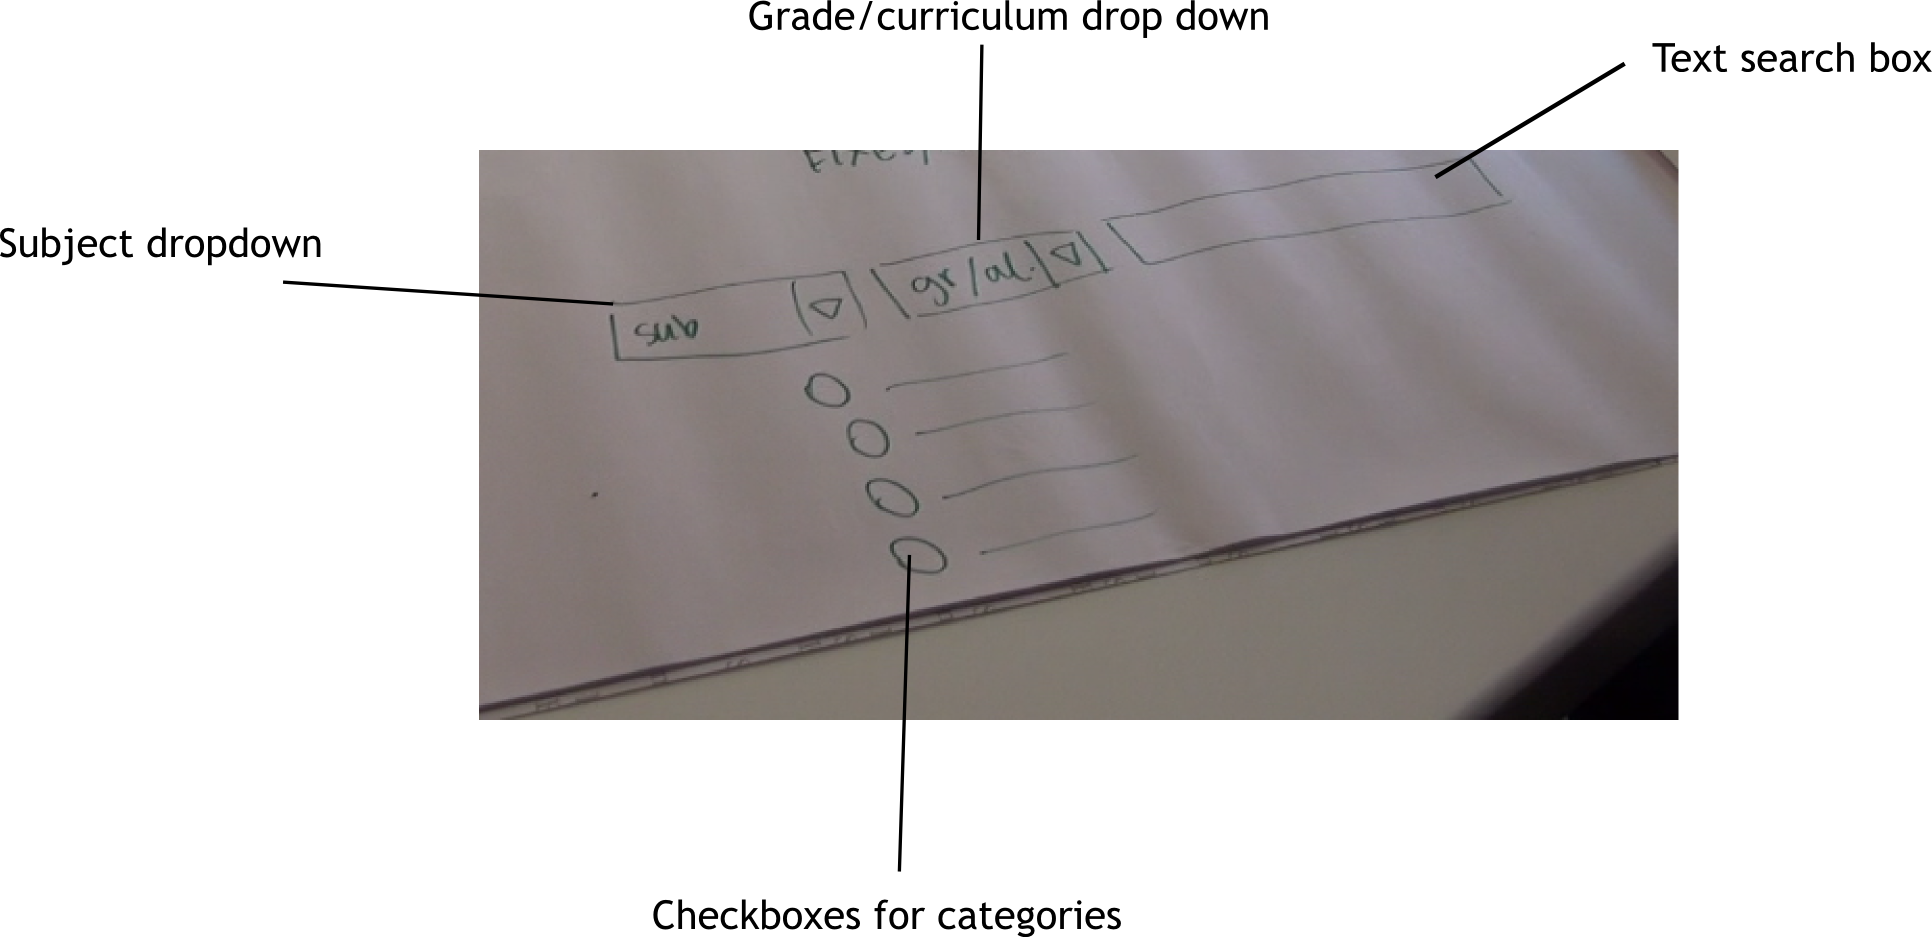
\includegraphics[width=\textwidth]{Figures/PD1shot2labels.png}
 \caption{Participants' initial drop-down interface idea}
\end{figure}

Participants suggested drop-down lists for high-level fields (subject, grade, curriculum) with a text search box. A checkbox list for the type of annotation (suggestion, errata, comment) was also suggested.

It was agreed that there would be value in starting with a broad overview of annotations and then refining the list of annotations based on filtering. This lead to the suggestion (from a "Development" user) that all annotations should be loaded into the browser as a default view (on first load).

\subsection{Second interface}
The second interface proposed by participants included a default view of all annotations (and any replies to them) listed in a table, in sortable columns including "date", "comment", "location" (URL) and so on. Users would then be able to refine their query using a combination of filters or facets on the left-hand side of the page. These filters would include subject, grade and category of annotation. Each set of filters would initially be visible but easily collapsible, so as not to take up too much screen real estate. Parameters within a filter would be selectable by checkbox lists (one or many could be selected simultaneously). Each set of filters would also have a "select all/none" checkbox, to avoid multiple clicking within a set of filters.
\begin{figure}[h!]
    \centering
    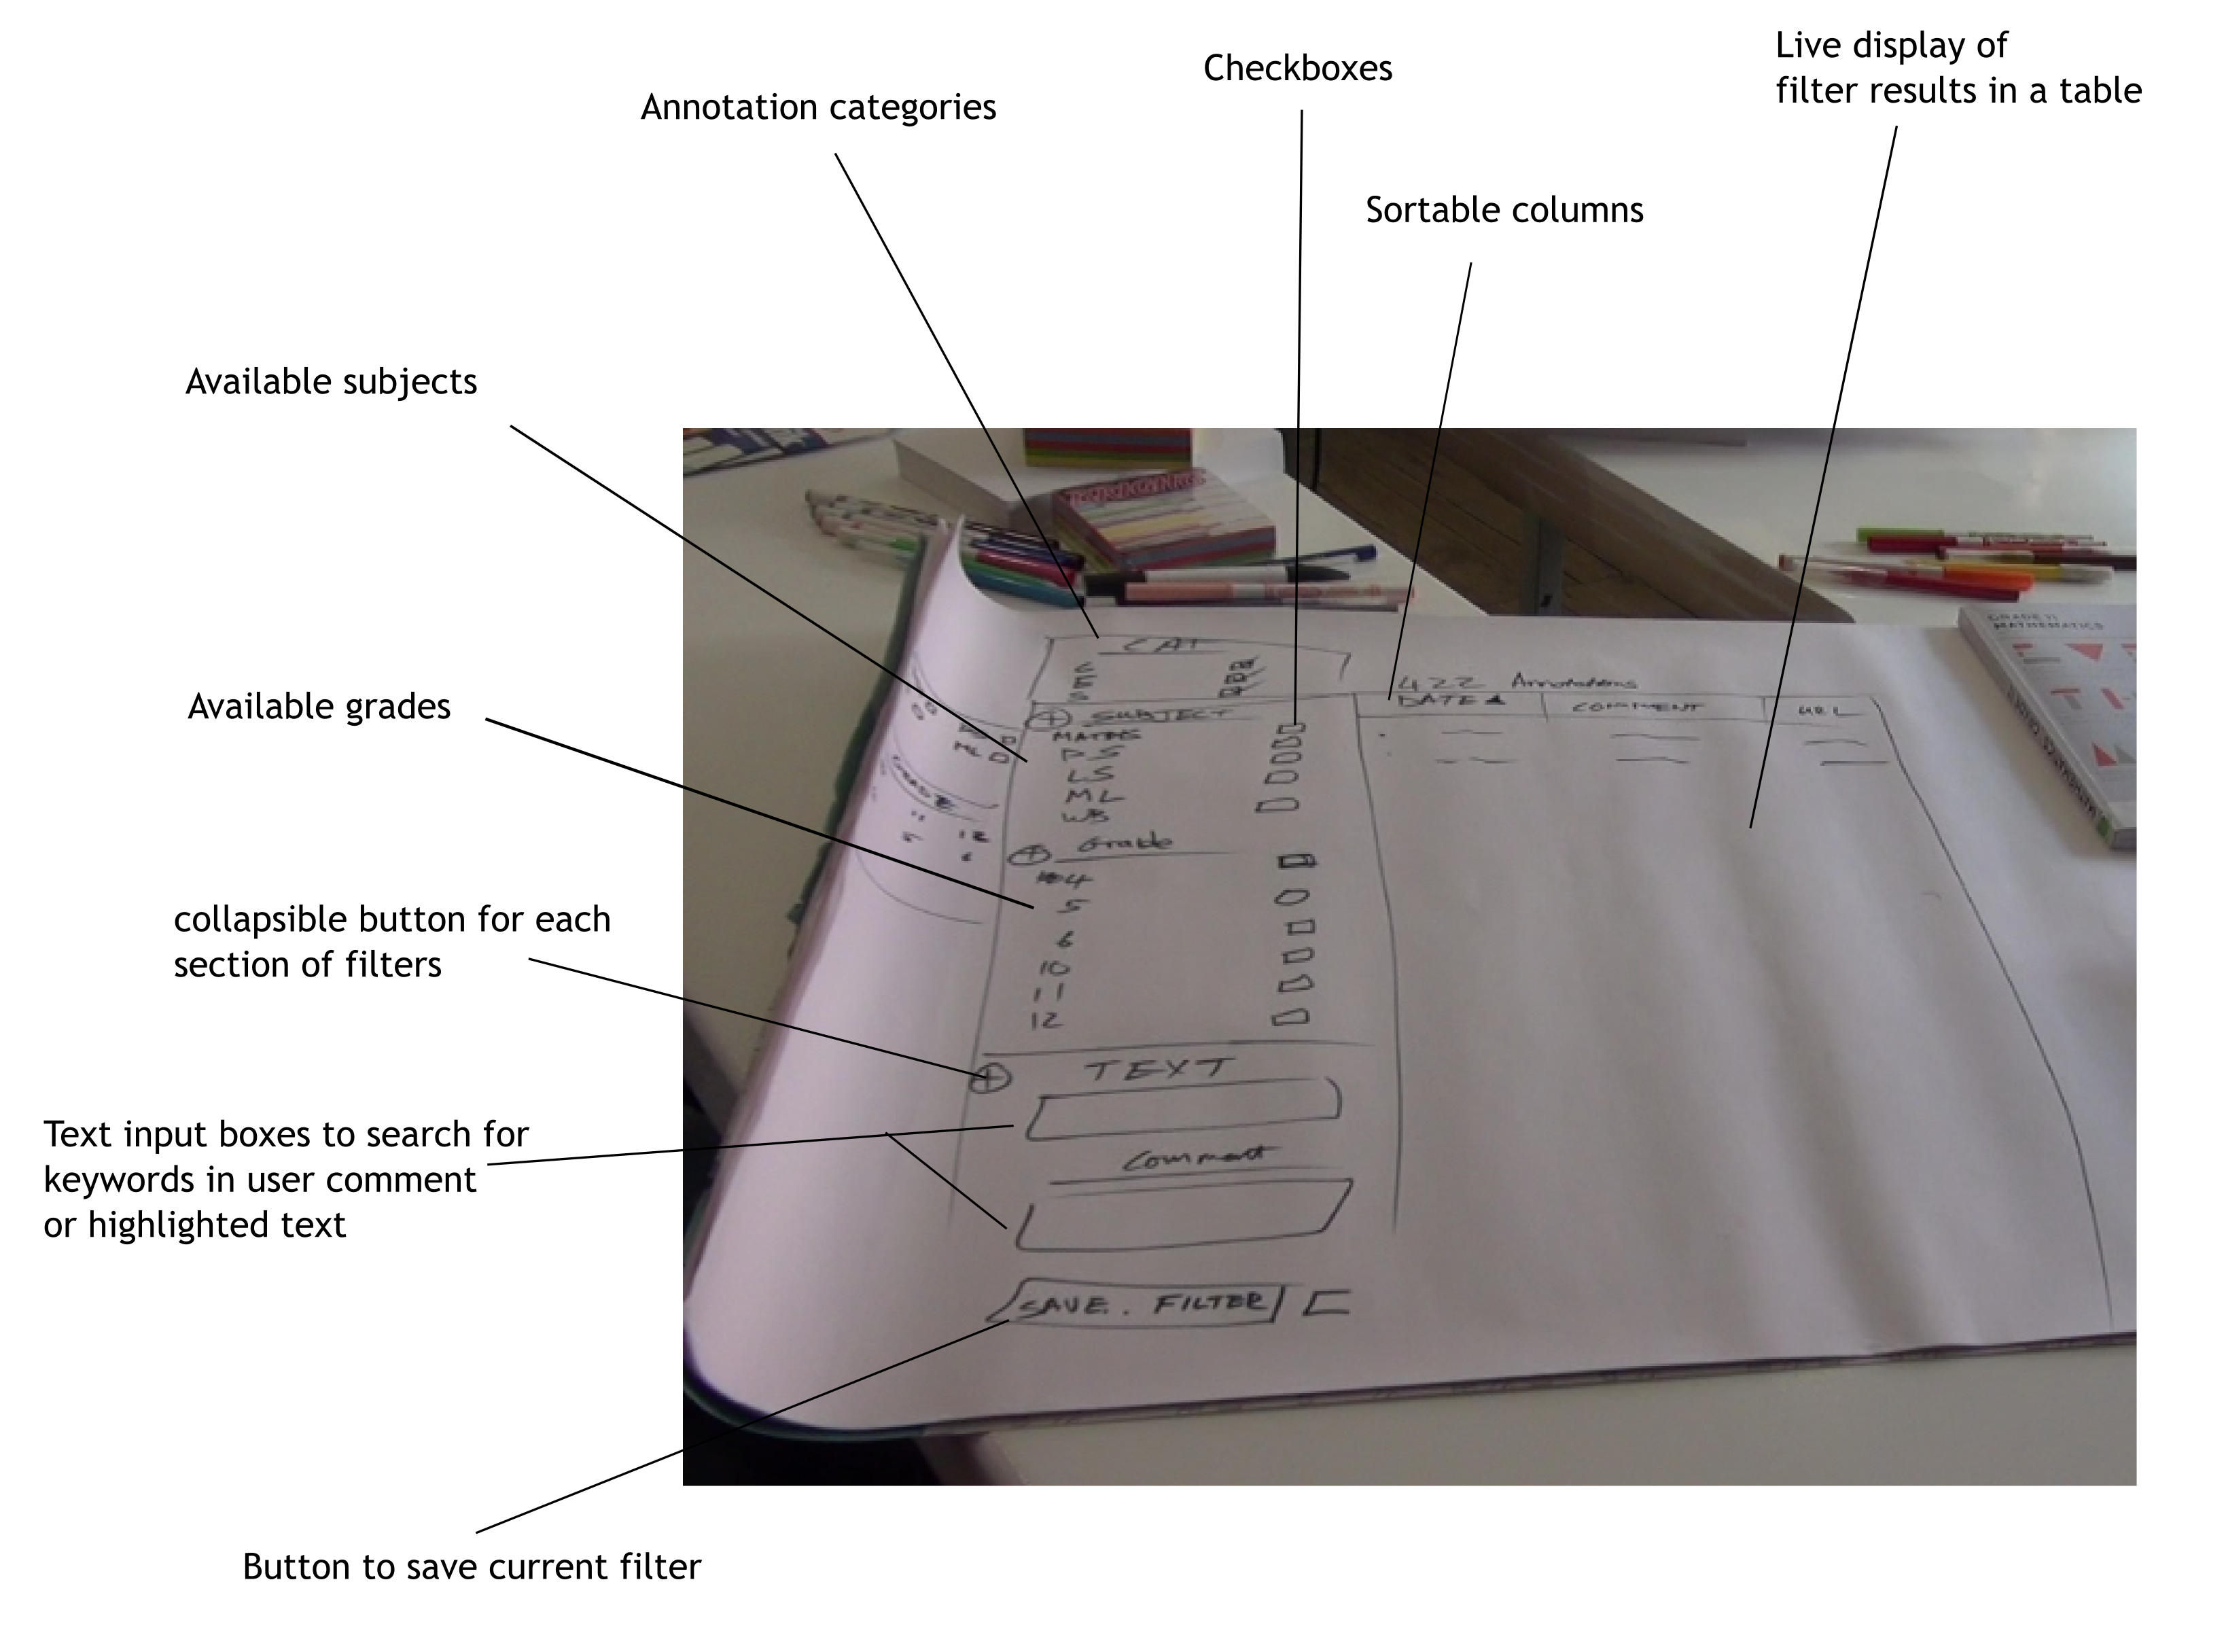
\includegraphics[width=\textwidth]{Figures/PD1shot4labels.png}
 \caption{Participants' second interface idea with filter/search options on the left and results on the right.}
\end{figure}

The inclusion of a text search box was suggested, to search for keywords in the user comment part of the annotation, or in the text being annotated. Whilst two text searches were initially suggested, participants later narrowed this down to one, that could search for text in either part of the annotation metadata. Being able to search by username (based on a pre-populated list) in this search box was also mentioned as being desirable functionality. 

\subsection{Behaviour}
In terms of behaviour,  the default view would include all annotations, and the list would be refined as participants clicked on different checkboxes and narrowed their results (e.g. if no specific grade was selected, annotations in all grades would be displayed). In the left-hand menu, the high-level filters (e.g. subject and grade) would initially be expanded, whilst the other lower-level sets of filters would be collapsed. It was suggested that the default view included greyed-out, selected checkboxes to indicate that all options were automatically selected. Clicking on one box would then select that box, and deselect the others. 

As filtering options were selected, the list of annotations displayed in the table of results (by date, with the most recent first) would then refresh in real time so that participants would have a continuous feedback loop between their filter selection and the search results. This would enable them to quickly refine their search based on the immediate displaying on results.

The live updating of results would eliminate the need for a "Search" or "Submit" button. However, it was agreed that if the database were to get very large (admittedly an unlikely scenario for the company at present, given that each annotation is just a few bytes of text data) it would be more efficient to have a static search with a "Submit" button which then returned results, otherwise the website would get very slow. 

It was agreed that it would be useful to be able to select how many results will be displayed per page (e.g. Wikipedia's "Next $\vert$ 20 $\vert$ 50 $\vert$ 100" \citep{Wikipedia}) to prevent unlimited scrolling through results. "Previous $\vert$ Next" breadcrumbs would also be useful for navigation between pages of tabulated results. 

\subsection{Saving filters and a user's last view}
Participants initially agreed that it would be useful to have an option to save specific queries, which could be loaded from a drop-down list. The saving of a specific combination of filters should include the option to give that query a name. The drop-down list of saved queries should include the query's name, the date on which it was saved, and the option to delete it.

If a saved query was selected, the associated checkboxes in the filter menu should automatically be populated. Users would then be able to select or deselect items to further refine their results.

It was agreed that the browser should remember a user's last selection of filters. Whether a user logged out and in again, or simply moved to another page and hit the "Back" button in their browser, they should immediately view the last list of results (and associated filters/selections).

Participants suggested a "Reset" or "Clear all" button to return to a default overview of all annotations. 

\subsection{Issue tracking}
Participants initially decided that it would be useful to have some mechanism by which annotations could be marked as "new" or "resolved", and be assigned to different team members for processing. This lead to a lengthy conversation about how the interface could possibly function as a skin for issue tracking software like GitHub or BitBucket. It was agreed that it would be useful to be able to set the status of an annotation, and to view said status in the results table. Resolved annotations should be listed last, or one should be able to easily exclude them from results, although they should not be deleted from the database.

\section{Session 2}
The second session focused on how participants would want their filtered results displayed, and how they would like to be able to sort those results. Many ideas were discussed and some ideas from the first session were refined, based on decisions and opinions about the table of displayed results. 

Following on from the issue tracking discussion in the first session, participants focused on being able to assign an annotation a "status" and a "person responsible". These fields were initially included in the table of displayed results. A tabbed table view was suggested, with "unassigned" issues as one tab, "busy-being-dealt-with" issues as a second tab and "resolved" issues as a third tab (much like the GitHub web interface). 

At some point in the second session however, one of the participants who is also a software developer pointed out that the group was no longer thinking about annotations - instead they were thinking about issues (in the bug tracking sense of the word). Issue tracking was then discarded by the participants as being too complex because it would mean a rework of the entire system, to design an interface between the annotator software and an issue tracker like RoundUp or GitHub. They then narrowed the paper prototype down to a more simple design, excluding the tabbed view and table columns that would indicate issue status and the responsible user. This was the only example of a significant discrepancy between participant opinions. 

\subsection{Displaying results}
After further discussion, participants agreed that results should be displayed in a table with the following sortable columns:\\ 
Category $\vert$ Info (URL, comment, highlighted text preview) $\vert$ Number of replies $\vert$ Date.

The default sort would be by date, with the most recent annotations listed first. The category column would include a visual representation of the type of annotation (comment, suggestion, errata), using coloured symbols to indicate type. This column would have a repetitive, circular sort, so one click would push one type of annotation to the top of the table, a second click would push the next type to the top and so on. 

The "Info" column would be sortable by URL (which means that annotations would essentially be sortable by section in the book, given the nature of the URLs). This column would display (vertically) a preview of the URL, the user comment made in the annotation and the text that the user highlighted. The URL would be hyperlinked to the original page on which the annotation was made. 

It was decided that "number of replies" was a useful category because an annotation with many replies is likely to need more urgent attention and processing than an annotation with no replies (e.g. if many users agree upon an erratum).

\subsection{Detailed results}
Participants discussed how the system should behave when a user clicks on a specific result listing or row. It was agreed that clicking on a table row should open a detailed view of that annotation that included all of the information about that annotation, the full URL, comment and highlighted text. This detailed view would open in the same window or frame. It would feature a back button, to return to the search results. Clicking on the URL would take the user to the original page in which the annotation was made for a contextualised view. 

\subsection{Refined filters}
Based on the results columns, the left-hand menu was then refined to contain only the following filters:
\begin{itemize}
\item subject
\item grade/alignment
\item chapter
\item category (Type of annotation)
\item username search box 
\end{itemize}

It was agreed that a top-down filter selection would need to be done. For example, the grades available depend on the subject selected, and similarly, the number of chapters available depend on the subject and grade selection. Participants decided that the dependent filters should populate automatically as the selection is refined. So once a user selects a particular subject, the list of available grades changes automatically to correspond with what books are available. 

Participants decided to eliminate the keyword text search box from the first session (they believed it would not be that useful), and instead have a username search box, that worked like an auto-complete search (so that internal users would not have to remember external usernames or worry about misspelling them). 

The option to save filters was discarded based on the new, simplified list of left-hand menu filters. Participants agreed that as long as their previous set of filters was saved (using cookies) when they returned to the site, that should be sufficient because the list of possible filters was now much shorter. 

\section{Consolidated prototype}
At the end of the second session, participants consolidated their ideas into the final paper prototype depicted in Figure \ref{fig:FinalPP}.
\begin{figure}[h!]
    \centering
    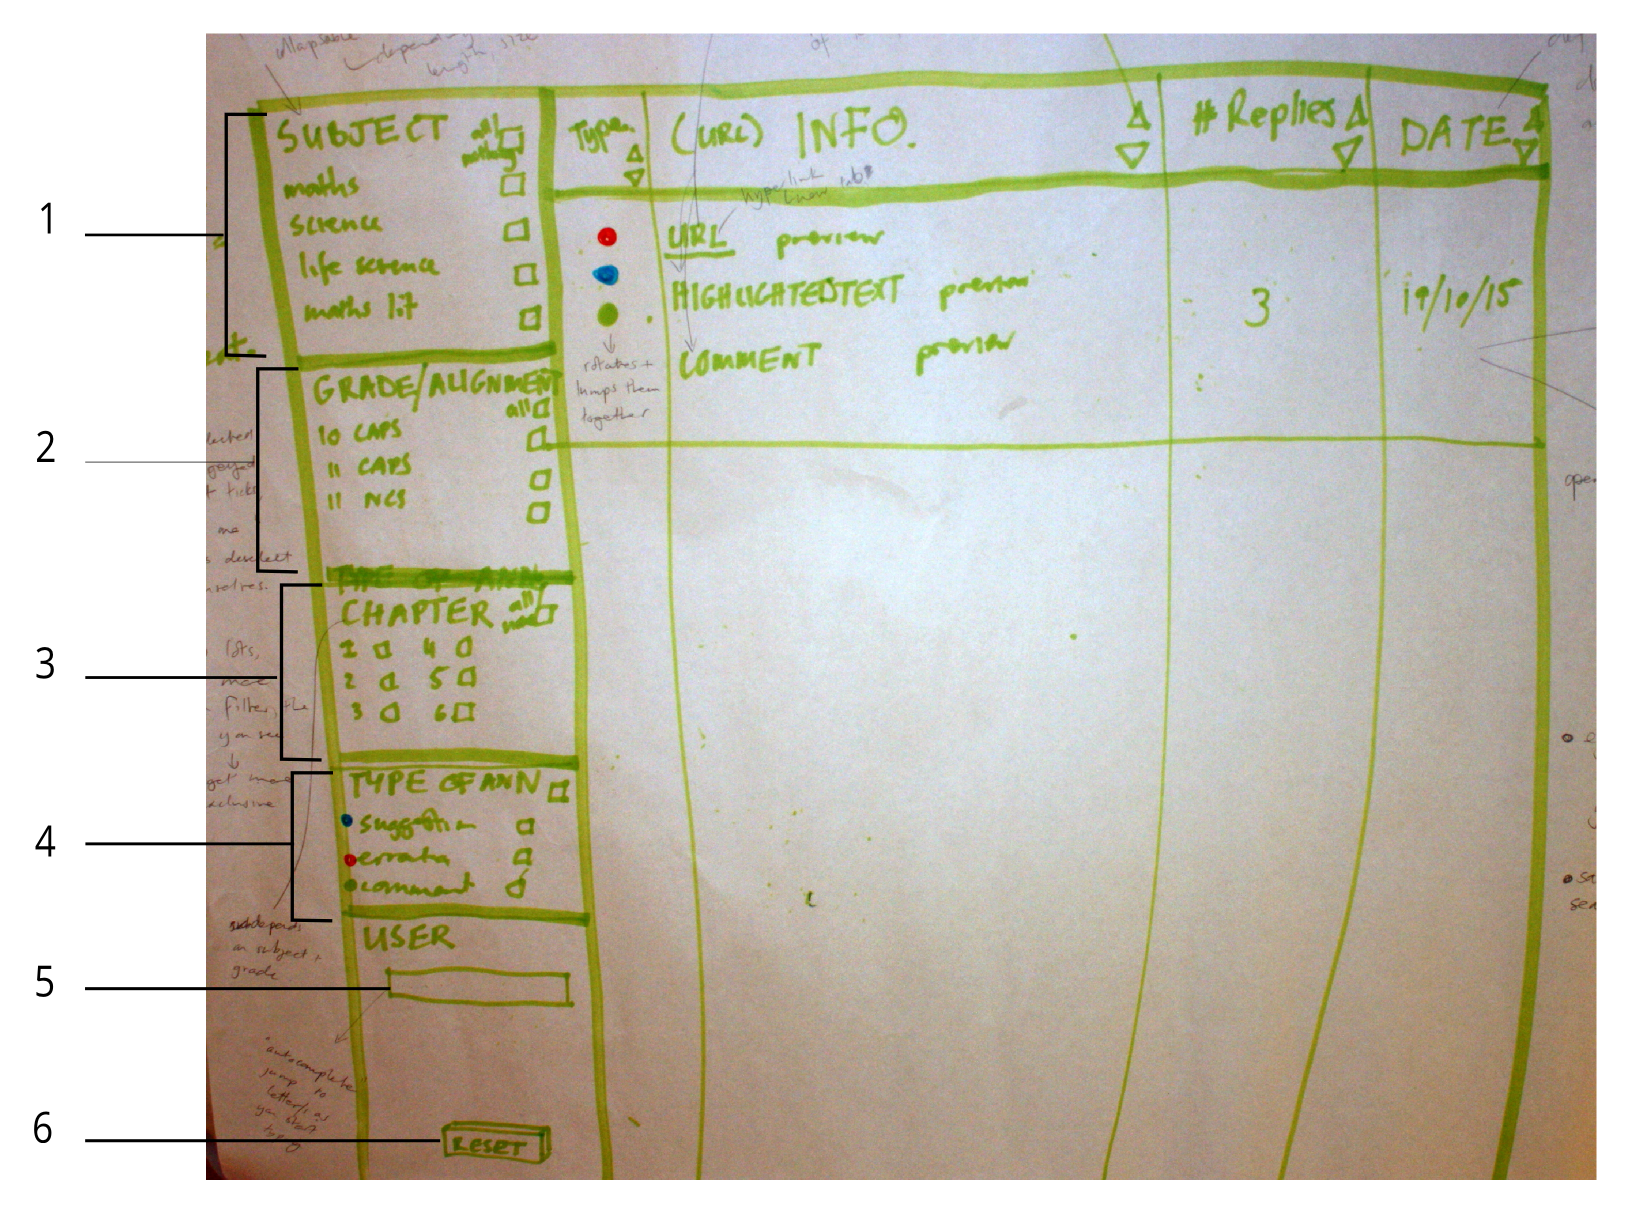
\includegraphics[width=\textwidth]{Figures/PDFinalLabels.png}
 \caption{The final paper prototype.}
 \label{fig:FinalPP}
\end{figure}

\subsection{Description of interface}
The interface would be divided into two main segments: a list of filters on the left-hand side of the page with a table of results taking up the rest of the page. At first login, the user would see the following filter options (see Figure \ref{fig:FinalPP}):
\begin{enumerate}
 \item subject
 \item grade/alignment 
 \item chapter
 \item type (of annotation - errata, suggestions etc.)
 \item username search box
 \item reset button (to return to default filter state)
\end{enumerate}

Everything would be expanded, and everything would be selected (so all annotations would be displayed initially). The fact that everything is automatically selected would be indicated by greyed-out, ticked, checkboxes. Each set of filters would be collapsible, and each would have a "select all/none" button. Clicking on one filter option (e.g. Subject = "Maths") would automatically deselect the other options. 

Lower-level filter options would automatically change based on higher level selections. (E.g. currently there only exists a Maths Literacy book for Grade 10, so if a user selects "Maths Literacy" as the subject filter, they should only see "Gr 10 CAPS" as an option under the grade filter). 

\begin{figure}[h!]
    \centering
    \includegraphics[width=0.6\textwidth]{Figures/PDfiltersLabels.png}
 \caption{Filter boxes in the final paper prototype.}
 \label{fig:FilterBoxes}
\end{figure}

The basic behaviour is that the user would initially see all the available annotations, and that "the more they click, the less they would see". So selecting filter options would refine the results displayed (live) in the table on the right. 

As mentioned above, the username search box would function like an auto-complete search, querying the database of known usernames as a user starts typing. A "Reset" or "Clear" button (Label 6 in Figure \ref{fig:FinalPP}) would be placed at the bottom of the left-hand options to return the displayed results to the default view. 

The table of displayed results would have the following sortable columns (see Figure \ref{fig:TableHead}): \\
$\vert$ Type $\vert$ Info (URL, comment \& highlighted text previews) $\vert$ Number of replies $\vert$ Date $\vert$\\
\\
\begin{figure}[h!]
    \centering
    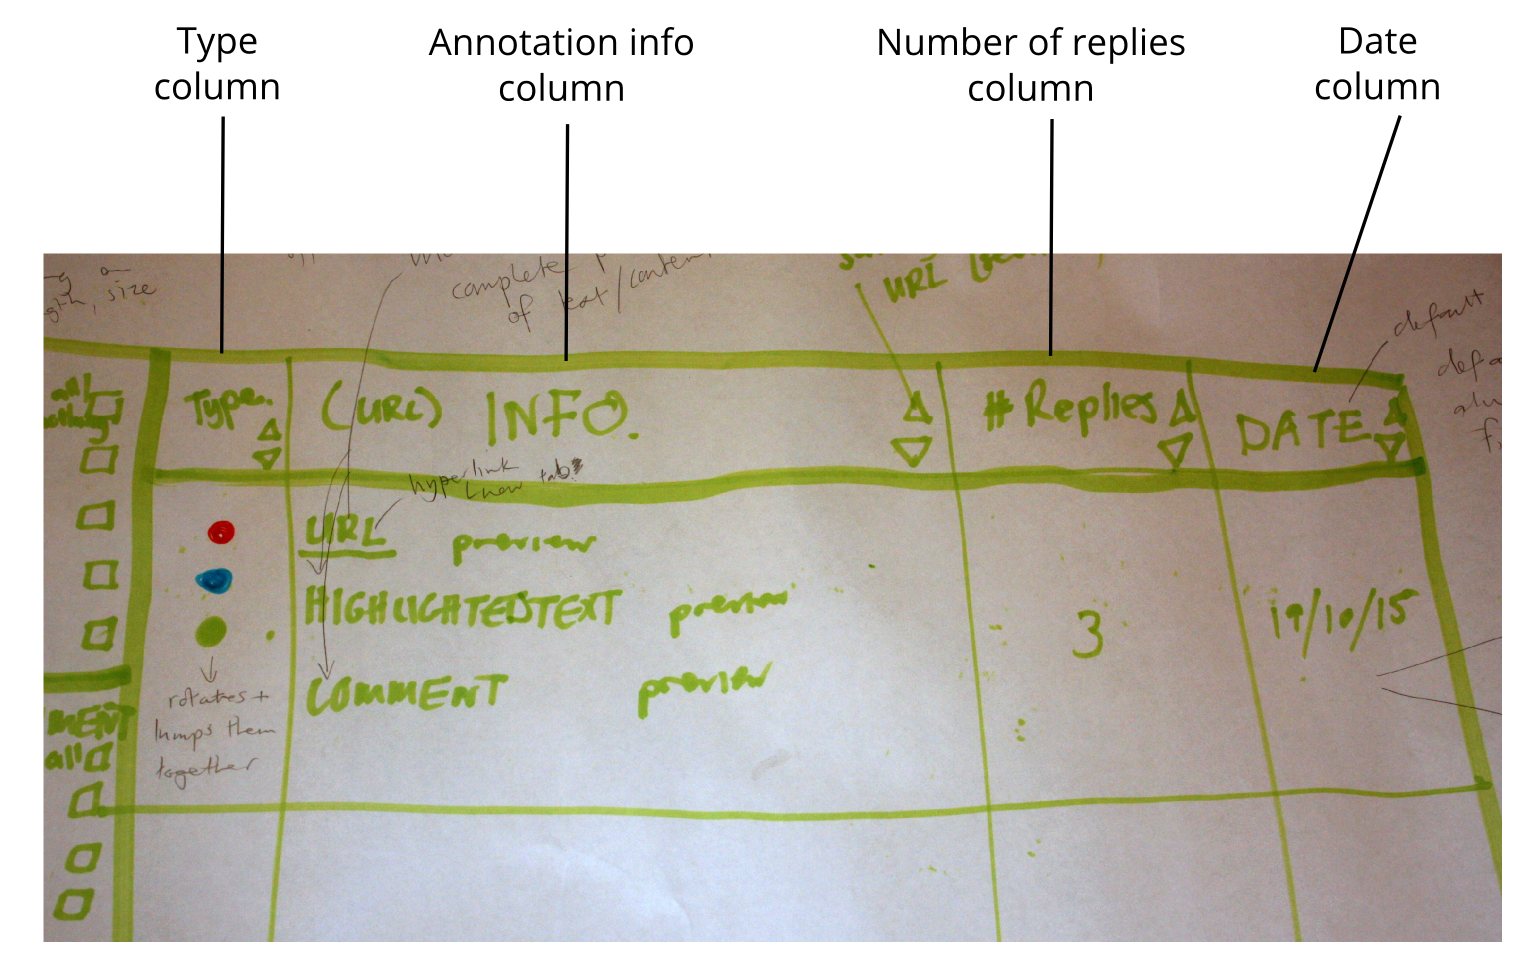
\includegraphics[width=\textwidth]{Figures/PDColumnHeadingLabels.png}
 \caption{Table heading columns in the final paper prototype.}
 \label{fig:TableHead}
\end{figure}
The default sort would be by date, with the most recent annotations listed first. The URL would hyperlink to the actual annotation in the book and the "Info" column would be sortable by URL (which corresponds to books and their chapters and sections). Breadcrumbs like $\vert$ Previous $\vert$ Next $\vert$ 20 $\vert$ 50 $\vert$ 100 $\vert$ would occur at the bottom of the table of results. 

The type of annotation would be indicated in the leftmost column by a small coloured icon. This column would sort in a rotational manner. 

Clicking on a particular annotation would open a detailed view of said annotation in a window (or frame) in the same page (see Figure \ref{fig:detailedoverlay}). Right-clicking a particular annotation would allow the user to open it in a new tab. This detailed view would contain all the available information about the annotation (full URL, comment, highlighted text, username, date, replies), and the hyperlinked URL to take one quickly to the original annotation in the context of a book.
\begin{figure}[h!]
    \centering
    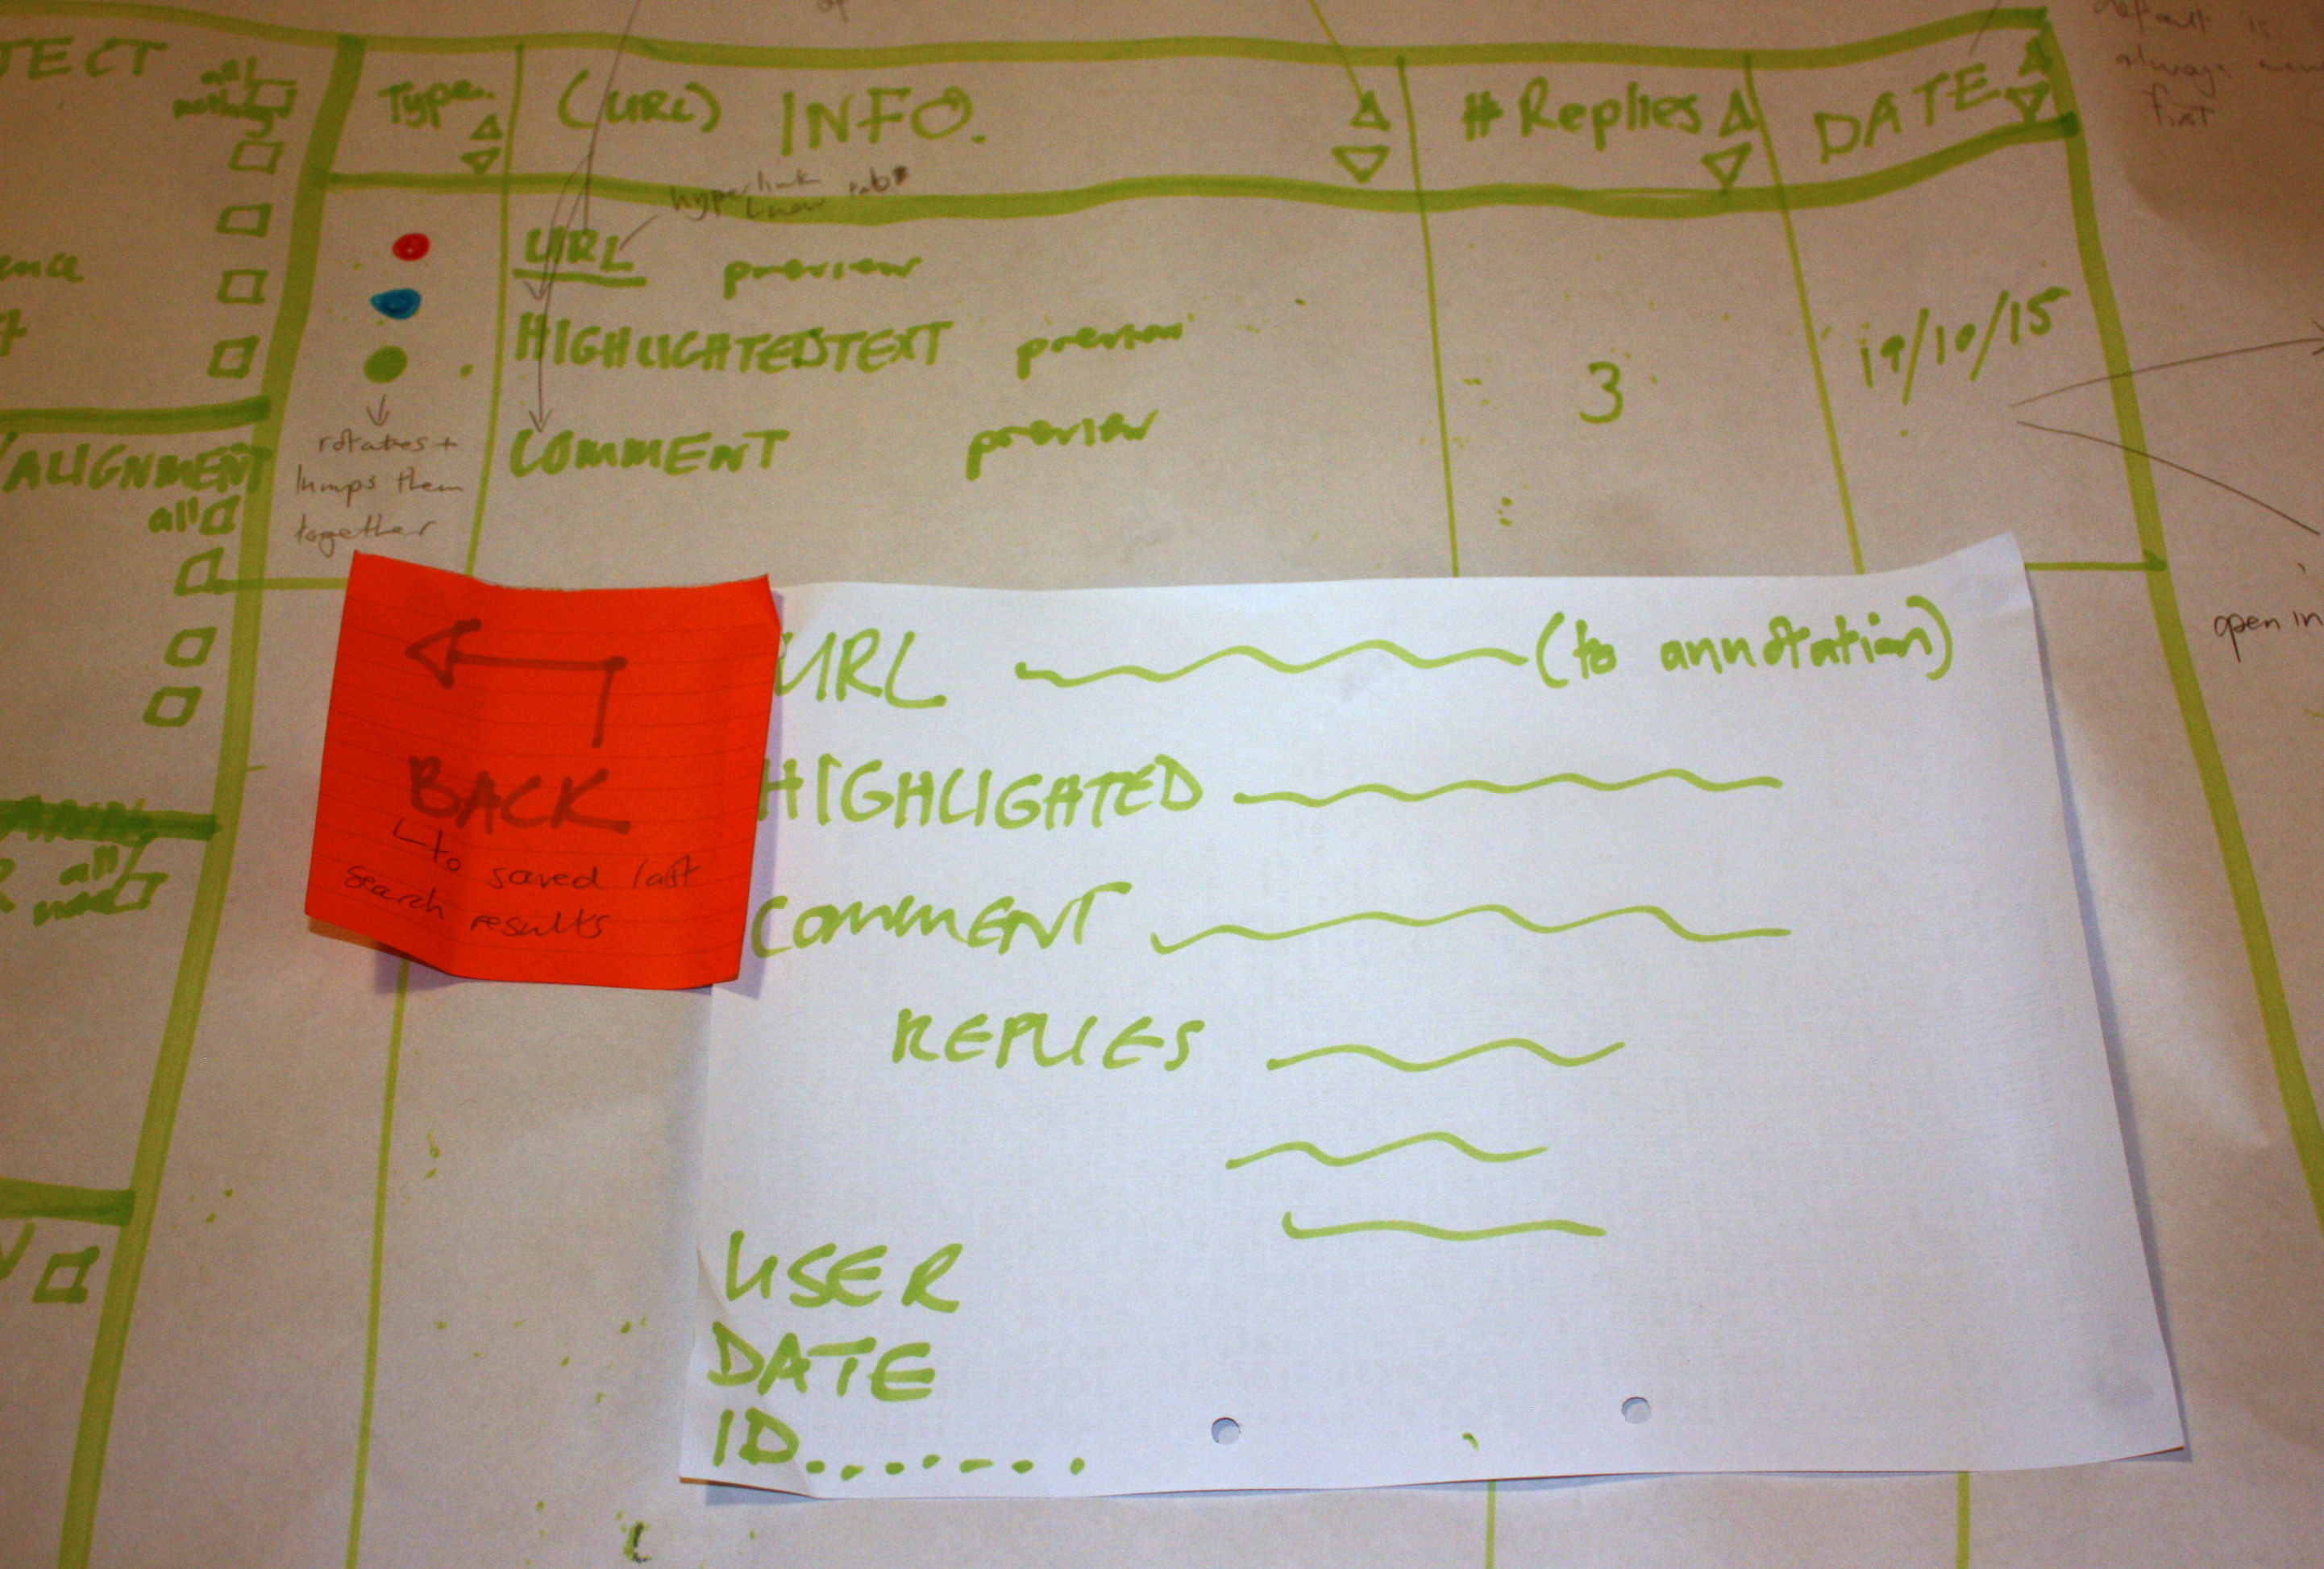
\includegraphics[width=\textwidth]{Figures/IMG_9044.JPG}
 \caption{Detailed view overlay in the final paper prototype.}
 \label{fig:detailedoverlay}
\end{figure}
\\
\\
Clicking "Back" from the detailed view would take users back to their previous set of filters and results. Likewise, if a user logged out and in again, or navigated back to the back-end interface from another page, they would see their last search results. 

\section{Discussion}
Overall, the participatory design process was constructive and informative. It was extremely valuable to get participants' input and having them work in a group together meant that they could discuss and refine ideas with each other and reach a unified design concept which satisfied everyone. 

Drawing several iterative sketches of the interface enabled participants to explore and experiment with different possibilities together. These sketches also seemed to help participants visualise concepts and explain ideas to each other. Whilst some participants were more comfortable talking than drawing, the group collectively struck a balance between thinking out loud and visualizing their ideas on paper for others to see.

Many ideas were brainstormed and then included or discarded as the participants' design evolved. These included different filter options (e.g. the keyword search, which was discarded later on), layout options (e.g. participants experimented with a tabbed table, and with drop-down filters before they decided on the left column layout), table heading options and assorted interface behaviours (e.g initially participants suggested collapsible filter sections, but later discarded this idea once they'd narrowed down the list of filter options and determined that they could probably all fit in the same view even if they were expanded).  

Because participants were used to brainstorming processes in the workplace, they were generally open to each other's suggestions and criticisms and there was little discrepancy between participants ideas and suggestions, with the exception of the issue tracking question. 

Having two separate sessions spaced one week apart also gave participants an opportunity to mull over ideas that had been discussed before the second session. 

Sometimes the brainstorming became very creative and extended beyond the scope of the interface in question. In these instances it  was challenging to try and keep participants focused on the task at hand, without dampening their enthusiasm. 

While the paper prototype seemed like a viable design solution that would thoroughly address user requirements, ultimately any proposed functionality that required issue tracking integration (e.g. GitHub) or server-side processing had to be excluded. This was in order to limit the scope of the project slightly and focus on the interface functionality itself, instead of the design of a database system that would have to include user authentication, server integration and so on. 
